\documentclass[ignorenonframetext,red]{beamer}

\usepackage{ucs}
\usepackage{mathpartir}
\usepackage{amsfonts,amsmath,amscd}
\usepackage{stmaryrd}
\usepackage[utf8x]{inputenc}
\usepackage[protrusion=true,expansion=true]{microtype}
\usepackage{setspace}
\usepackage{graphicx}
\usepackage{natbib}
\usepackage{listings}

\date{\\[1em]$\star$ January 2011 $\star$\\[1em]
\scriptsize PPS -- Groupe de travail théorie des types et réalisabilité}

\title{A logical framework for incremental type-checking}

\author[Matthias Puech \& Yann Régis-Gianas] {
  Matthias Puech\inst{1,2} \and Yann Régis-Gianas\inst{2}
}

\institute {
  \inst 1 {Dept. of Computer Science, University of Bologna} \and
  \inst 2 {University Paris 7, CNRS, and INRIA, PPS, team ${\pi}r^2$}
}

\setbeamertemplate{footline}[frame number]
\setbeamertemplate{navigation symbols}{}

\usefonttheme{serif}

\AtBeginSection[]
{\begin{frame}<beamer>{Menu}
    \tableofcontents[currentsection]
  \end{frame}
}

% Grammars
\newcommand\gor{\ |\ }
\newcommand\gequal{\ ::=\ }

% Terms
\newcommand\postbinder{\cdot}
\newcommand\prd[2]{\ensuremath\Pi{#1}^{#2}\postbinder}
\newcommand\prdi[1]{\ensuremath\forall{#1}\postbinder}
\newcommand\app[1]{{#1}\ }
\newcommand\tlam[2]{\ensuremath\lambda{#1}^{#2}\postbinder}
\newcommand\ulam[1]{\ensuremath\lambda{#1}\postbinder}
\newcommand\letb[2]{\ensuremath\mathsf{let}\ {#1}={#2}\ \mathsf{in}\ }
\newcommand\lam{\tlam}

% Sorts
\newcommand\srt[1]{\ensuremath\mathsf{#1}}
\newcommand\type{\srt *}
\newcommand\kind{\srt \Box}

% Sequent-like application
\newcommand\lapp[2]{{#1}[{#2}]}
\newcommand\laapp[3]{{#1}[{#2}]:{#3}}
\newcommand\lnil{\cdot}
\newcommand\lcons[2]{{#1};{#2}}
\newcommand\lncons[3]{{#1}={#2};{#3}}

%Environments
\newcommand\enil\cdot
\newcommand\eent[1]{\left[{#1}\right]}
\newcommand\econs[2]{{#1}\eent{#2}}
\newcommand\esing[1]{\econs{}{#1}}
\newcommand\emerge[2]{{#1}\cdot{#2}}
\newcommand\elookup[2]{{#1}({#2})}
\newcommand\elookupdef[3]{{#1}({#2}) = {#3}}
\newcommand\elookupdecl[3]{{#1}({#2}) : {#3}}
\newcommand\ebind[2]{\econs{#1}{#2}}
\newcommand\ebinddef[3]{\econs{#1}{{#2}={#3}}}
\newcommand\ebinddecl[3]{\econs{#1}{{#2}:{#3}}}
\newcommand\edecls[1]{\mathsf{decls}({#1})}
\newcommand\edefs[1]{\mathsf{defs}({#1})}


% Term operations
\newcommand\subst[2]{\{{#1}/{#2}\}}
\newcommand\repl[2]{\subst{#1}{{#2}}}
\newcommand\conv{\equiv}

% Judgements
\newcommand\jlang[3]{{#2}\vdash_{\mathrm{#1}}{#3}}
\newcommand\jlangt[4]{{#2}\vdash_{\mathrm{#1}}{#3}:{#4}}
\newcommand\jlangA[3]{{#2}\vdash_{\mathrm{#1}}{#3}\mathsf{\ type}}
\newcommand\jlangK[3]{{#2}\vdash_{\mathrm{#1}}{#3}\mathsf{\ kind}}

\newcommand\jlft[3]{\jlangt{LF}{#1}{#2}{#3}}
\newcommand\jlfA[2]{\jlangA{LF}{#1}{#2}}
\newcommand\jlfK[2]{\jlangK{LF}{#1}{#2}}

\newcommand\jxlft[3]{\jlangt{XLF}{#1}{#2}{#3}}
\newcommand\jxlfA[2]{\jlangA{XLF}{#1}{#2}}
\newcommand\jxlfK[2]{\jlangK{XLF}{#1}{#2}}

\newcommand\jnlft[3]{\jlangt{}{#1}{#2}{#3}}
\newcommand\jnlfA[2]{\jlangA{}{#1}{#2}}
\newcommand\jnlfK[1]{{#1}\ \mathsf{kind}} %on peut pas utiliser \jlangK

\newcommand\jnlfargs[3]{\jnlft{#1}{#2}{#3}}
\newcommand\jnlfconvA[3]{\jnlfA{#1}{{#2}\conv{#3}}}
\newcommand\jnlfconvt[4]{\jnlft{#1}{{#2}\conv{#3}}{#4}}
\newcommand\jnlfconve[3]{\jlang{}{#1}{{#2}\conv{#3}}}

% simple judgements with no environments (NLF)
\newcommand\jwf[1]{{#1}\ \mathsf{wf}}

% Animations
\newcommand\alta[4]{\alt<-#1>{#3}{\alert<#2>{#4}}}
\newcommand\uncovera[2]{\uncover<#1->{\alert<#1>{#2}}}
\newcommand\onlya[2]{\only<#1->{\alert<#1>{#2}}}

% Various
\newcommand\gray[1]{\textcolor{gray}{#1}}
\newcommand\cit[1]{[\textcolor{blue}{#1}]}
\newcommand\To{\Rightarrow}
\newcommand\too{\longrightarrow}
\newcommand\Too{\Longrightarrow}
\newcommand\nat{\mathbb N}
\newcommand\FV[1]{\mathsf{FV}({#1})}
\newcommand\notinfv[2]{{#1}\notin\FV{#2}}

\newcommand\itplus{\textcolor{green!60!black}{\textbf{\textsf{+}}}}
\newcommand\itminus{\textcolor{red}{\textbf{\textsf{--}}}}

\newenvironment{smallright}{
  \begin{flushright}
    \footnotesize
  }{
  \end{flushright}
}

\lstset{
  language=[Objective]Caml,
  basicstyle=\sf,
  columns=flexible,
  literate={->}{{$\to$ }}1 {*}{$\times$ }1 {>=}{{$\geq$}}1
  {<>}{{$\neq$}}1 {'a}{{$\alpha$}}1 {'b}{{$\beta$}}1 {'c}{{$\gamma$}}1
}

\begin{document}

\frame\titlepage

\begin{frame}{A paradoxical situation}  
  \begin{block}{Observation}
    We have powerful tools to mechanize the metatheory of (proof) languages
  \end{block}
  \pause
  \begin{block}{\ldots\ And yet,}
    Workflow of programming and formal mathematics is still largely inspired by legacy
    software development (\textsf{emacs}, \textsf{make}, \textsf{svn},
    \textsf{diff}s\ldots)
  \end{block}
  \vspace{0.6em}
  \pause
  \begin{center}
    {\large \it Isn't it time to make these tools metatheory-aware?}
  \end{center}
\end{frame}

\begin{frame}{Incrementality in programming {\it \&} proof languages}
  
  {\Huge Q {\Large :}} \parbox{0.8\textwidth}{Do you spend more time
    \emph{writing} code or \emph{editing} code?} \\[2em]

Today, we use:
  \begin{itemize}
  \item separate compilation
  \item dependency management
  \item version control on the scripts
  \item interactive toplevel with rollback (\textsf{Coq})
  \end{itemize}
\end{frame}

\begin{frame}{Incrementality in programming {\it \&} proof languages}
  \vspace{0.5em}
  \begin{center}
    \only<1>{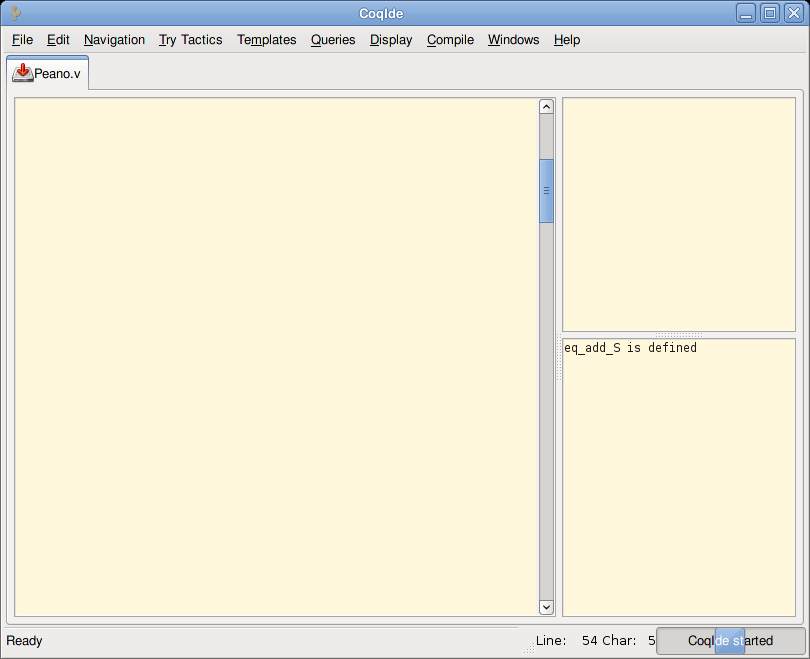
\includegraphics[width=0.85\textwidth]{images/coqide00.png}}%
    \only<2>{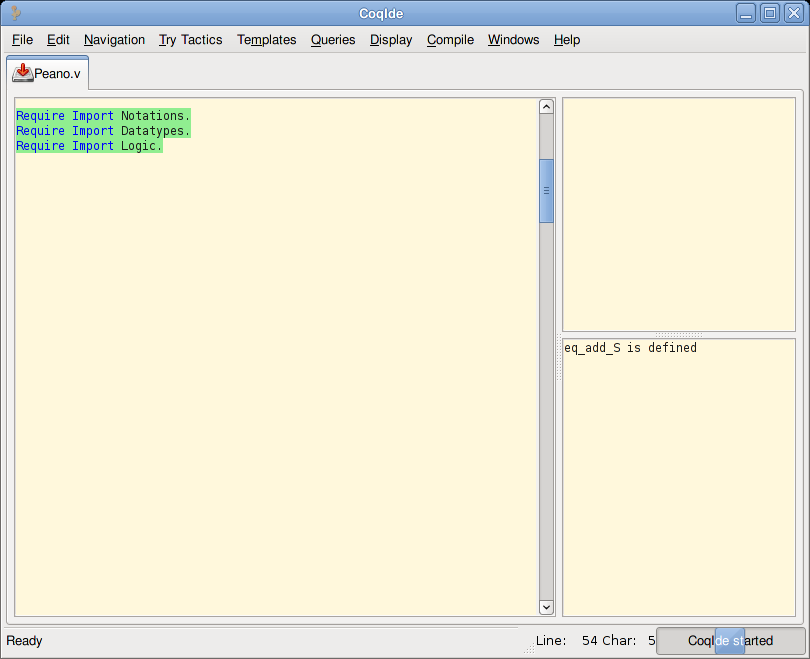
\includegraphics[width=0.85\textwidth]{images/coqide0.png}}%
    \only<3>{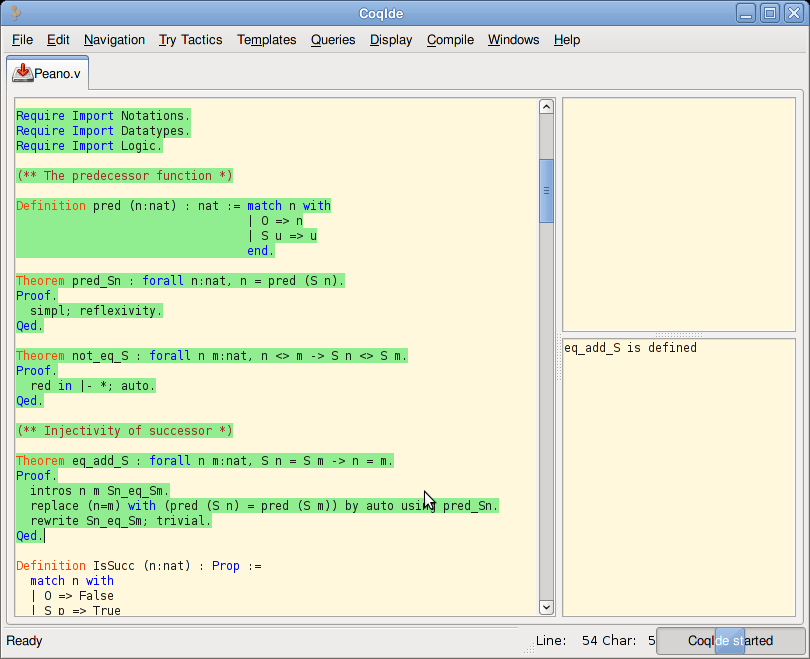
\includegraphics[width=0.85\textwidth]{images/coqide.png}}%
    \only<4>{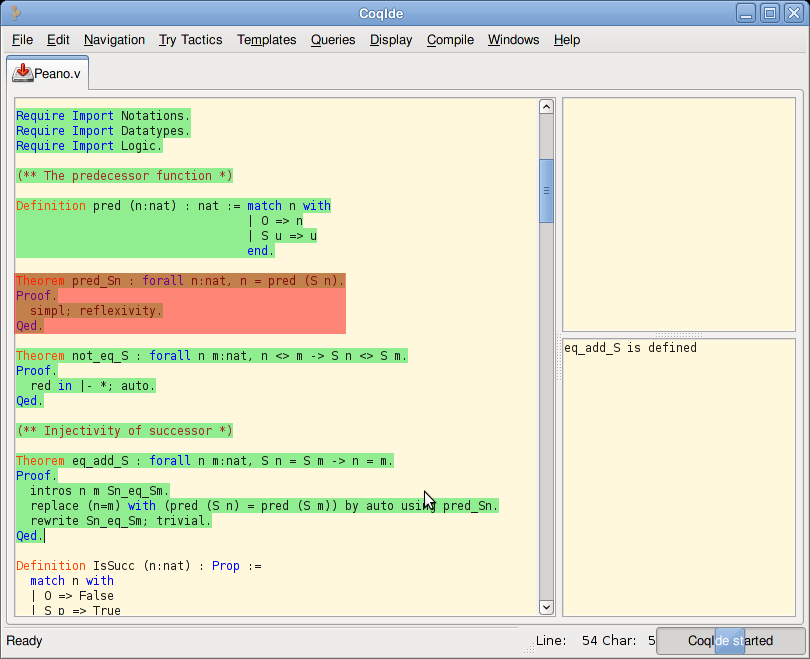
\includegraphics[width=0.85\textwidth]{images/coqide2.png}}%
    \only<5>{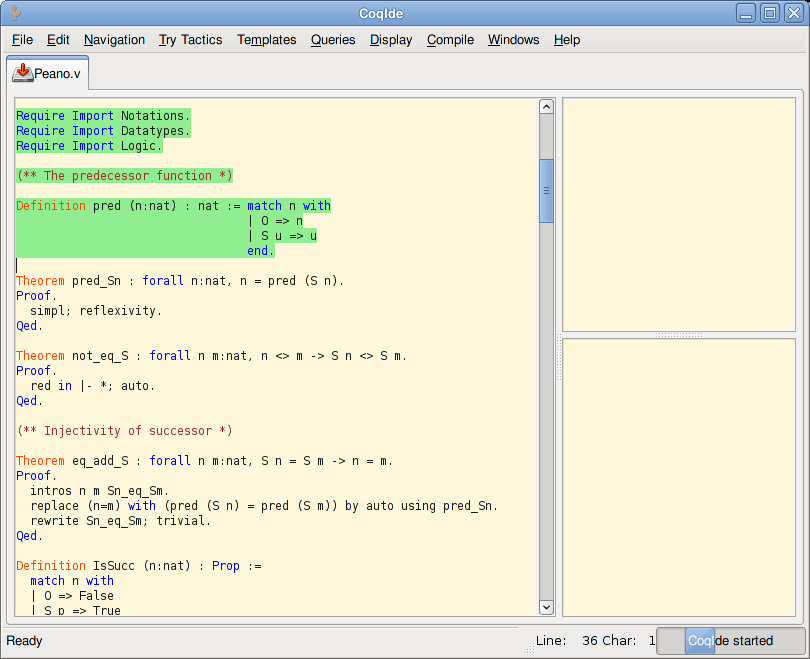
\includegraphics[width=0.85\textwidth]{images/coqide4.png}}%
    \only<6>{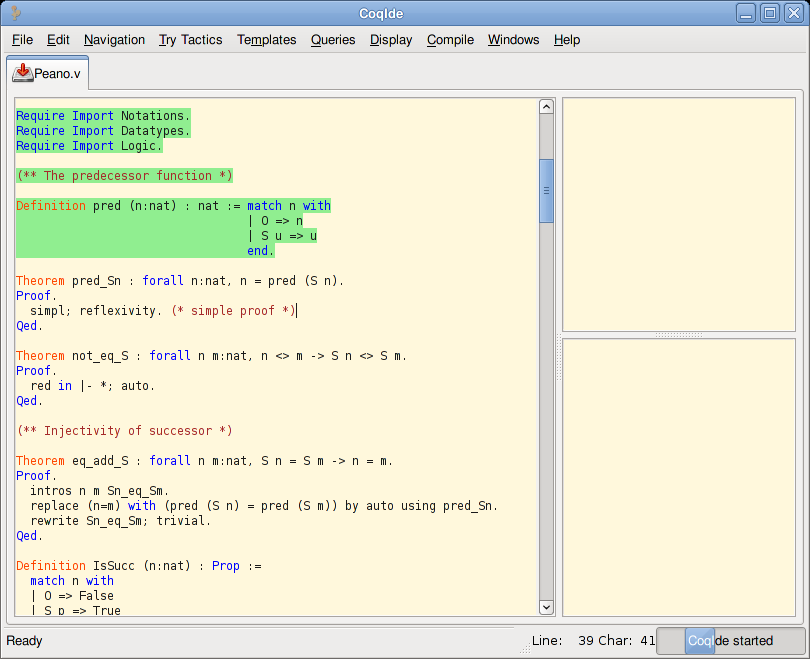
\includegraphics[width=0.85\textwidth]{images/coqide5.png}}%
    \only<7>{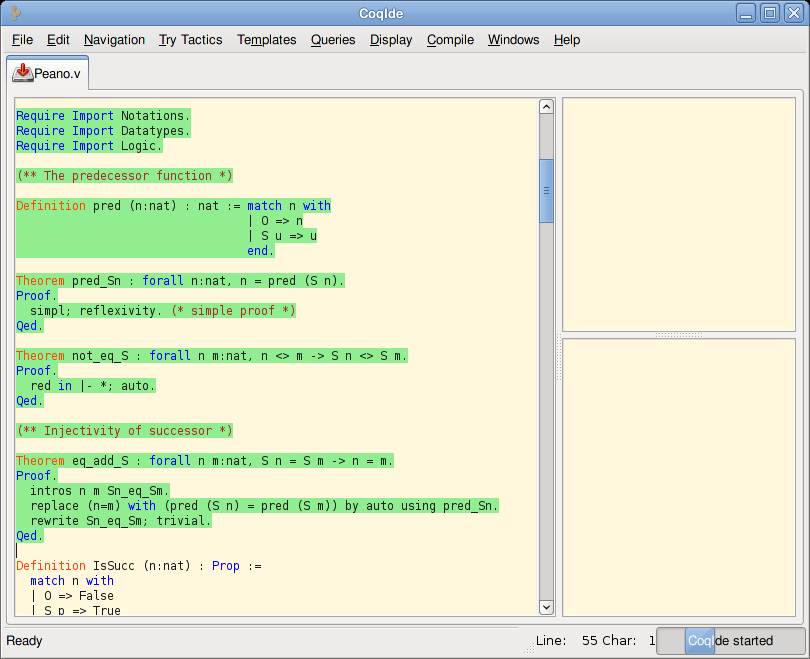
\includegraphics[width=0.85\textwidth]{images/coqide6.png}}%
    \only<8>{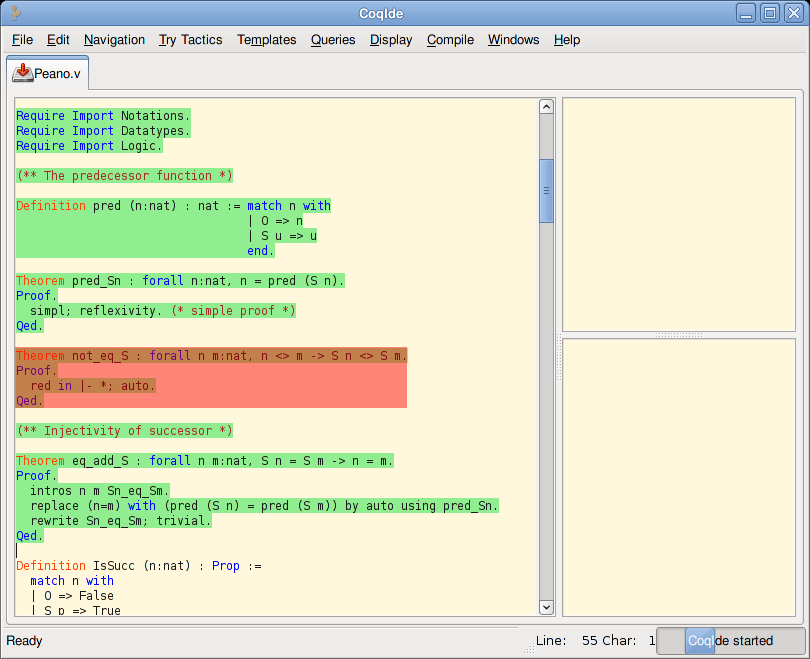
\includegraphics[width=0.85\textwidth]{images/coqide7.png}}%
  \end{center}
\end{frame}

\begin{frame}{In an ideal world\ldots}
  \begin{itemize}
  \item Edition should be possible anywhere
  \item The impact of changes visible “in real time”
  \item No need for separate compilation, dependency management
  \end{itemize}
  \pause
  \vspace{2em}
  \begin{center}
    {\Large \it Types are the witnesses of this impact}
  \end{center}
  \vspace{1em}
  \pause
  \begin{block}{Applications}
    \begin{itemize}
    \item non-linear user interaction
    \item dependency management
    \item type-directed programming
    \item typed version control systems
    \end{itemize}
  \end{block}

\end{frame}

\begin{frame}{Menu}
  \tableofcontents
\end{frame}

\section{The big picture}

\begin{frame}[fragile]{\gray{A logical framework for incremental}
    type-checking}
  Yes, we're speaking about (any) typed language.
  \begin{block}{A type-checker}
    \begin{lstlisting}
      val check : env -> term -> types -> bool
    \end{lstlisting}
    \begin{itemize}
    \item builds and checks the derivation (on the stack)
    \item conscientiously discards it
    \end{itemize}
  \end{block}
  \pause
  \def\envbarb{A\to B, B\to C, A\vdash}
  
  \begin{overlayarea}{\textwidth}{7em}
    \alt<-2>{
      \[ \tiny
      \def\impi{{\tiny$\to_i$}}
      \def\impe{{\tiny$\to_e$}}
      \def\ax{{\tiny$Ax$}}
      \infer*[left=\impi]{
        \infer*[left=\impi]{
          \infer*[left=\impi]{
            \infer*[left=\impe]{
              \infer*[right=\ax,leftskip=5em]{ }{\envbarb B\to C}\\
              \infer*[right=\impe,rightskip=5em]{
                \infer*[right=\ax]{ }{\envbarb A\to B}\\
                \infer*[right=\ax]{ }{\envbarb A}
              }{\envbarb B}
            }{\envbarb C}
          }{A\to B, B\to C\vdash A\to C}
        }{A\to B\vdash (B\to C)\to A\to C}
      }{\vdash (A\to B)\to(B\to C)\to A\to C}
      \]
    }{
      \begin{center}
        \vspace{3em}
        \large \textsf{\textbf{true}}
      \end{center}
    }
  \end{overlayarea}
  \pause  
\end{frame}

\begin{frame}{\gray{A logical framework for} incremental
    \gray{type-checking}}
  
\end{frame}

\begin{frame}{The big picture}
  \begin{center}
    \only<1-2>{\fbox{\parbox{20em}{\only<2>\alert{version
            management}\\[1em]%
          \fbox{\parbox{18em}{script files\\[1em]%
              \fbox{\parbox{17em}{parsing\\[1em]%
                  \fbox{\parbox{14em}{type-checking\\} }}}}}}}}%
    \only<3>{\fbox{\parbox{20em}{script files\\[1em]%
          \fbox{\parbox{18em}{\alert{version management}\\[1em]%
              \fbox{\parbox{17em}{parsing\\[1em]%
                  \fbox{\parbox{14em}{type-checking\\} }}}}}}}}%
    \only<4-6>{\fbox{\parbox{20em}{
          \begin{overlayarea}{20em}{2em}
            \alt<-5>{script files}{user interaction}
          \end{overlayarea}%
          \fbox{\parbox{18em}{parsing\\[1em]%
              \fbox{\parbox{17em}{\alert{version management}\\[1em]%
                  \uncover<4-6>{\fbox{\parbox{14.5em}{type-checking\\}}}}}}}}}}%
    \only<7->{\fbox{\parbox{20em}{
          \begin{overlayarea}{20em}{2em}
            user interaction
          \end{overlayarea}%
          \fbox{\parbox{18em}{parsing\\[1em]%
              \fbox{\parbox{17em}{\only<8->{incremental }type-checking\\[1em]%
                  \fbox{\parbox{14.5em}{\alert{version management}\\}}}}}}}}}%
  \end{center}
  \begin{itemize}
  \item<4-> AST representation
  \item<5-> Explicit dependency DAG
  \item<7-> Typing annotations
  \end{itemize}
\end{frame}

\section{Our approach}

\subsection{Why not memoization?}

\begin{frame}[fragile]{Memoization maybe?}
  \begin{onlyenv}<1>
    \vspace{4em}
\begin{lstlisting}
let rec check env t a = 
  match t with
  | ... -> ... false
  | ... -> ... true

and infer env t =
  match t with 
  | ... -> ... None
  | ... -> ... Some a
\end{lstlisting}
  \end{onlyenv}
  \begin{onlyenv}<2>
    \vspace{3em}
\begin{lstlisting}
let table = ref ([] : environ * term * types) in
let rec check env t a = 
  if List.mem (env,t,a) !table then true else
    match t with
    | ... -> ... false
    | ... -> ... table := (env,t,a)::!table; true
and infer env t =
  try List.assoc (env,t) !table with Not_found ->
    match t with 
    | ... -> ... None
    | ... -> ... table := (env,t,a)::!table; Some a
\end{lstlisting}
  \end{onlyenv}
  \pause\pause
  \begin{enumerate}[<+->]
  \item[\itplus] lightweight
  \item[\itplus] efficient implementation
  \item[\itminus] imperative (or untractable)
  \item[] \footnotesize What if I want \emph{e.g.} the weakening property to be taken into account?
  \item [\itminus] syntactic comparison
  \item[] \footnotesize What does it mean logically?
    \begin{mathpar}
      \infer
      {J\in \Gamma} 
      {\Gamma\vdash \jwf J\To \Gamma} \and
      \infer
      {\Gamma_1\vdash \jwf{J_1} \To \Gamma_2\\\ldots\\ \Gamma_{n-1}[J_{n-1}]\vdash
        \jwf{J_n}\To \Gamma_n}
      {\Gamma_1\vdash \jwf J\To \Gamma_n[J_n][J]}
    \end{mathpar}
  \item[\itminus] external to the logic (meta-cut)
  \item[\itminus] introduces a dissymmetry
  \item[\itminus] still no trace of the derivation
  \item[\itplus] gives good reasons to go on
  \end{enumerate}
\end{frame}

\subsection{A popular storage model for repositories}

\begin{frame}{A popular storage model for repositories}
  \begin{onlyenv}<1-7>
    \begin{center}
      \only<+>{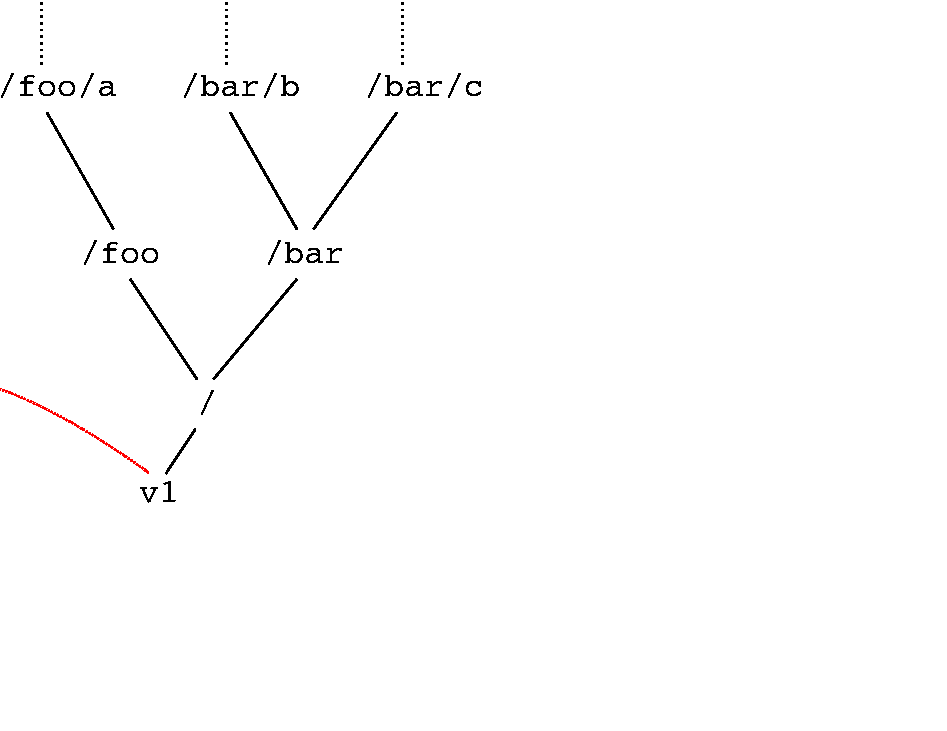
\includegraphics[width=0.85\textwidth]{images/git1.pdf}}%
      \only<+>{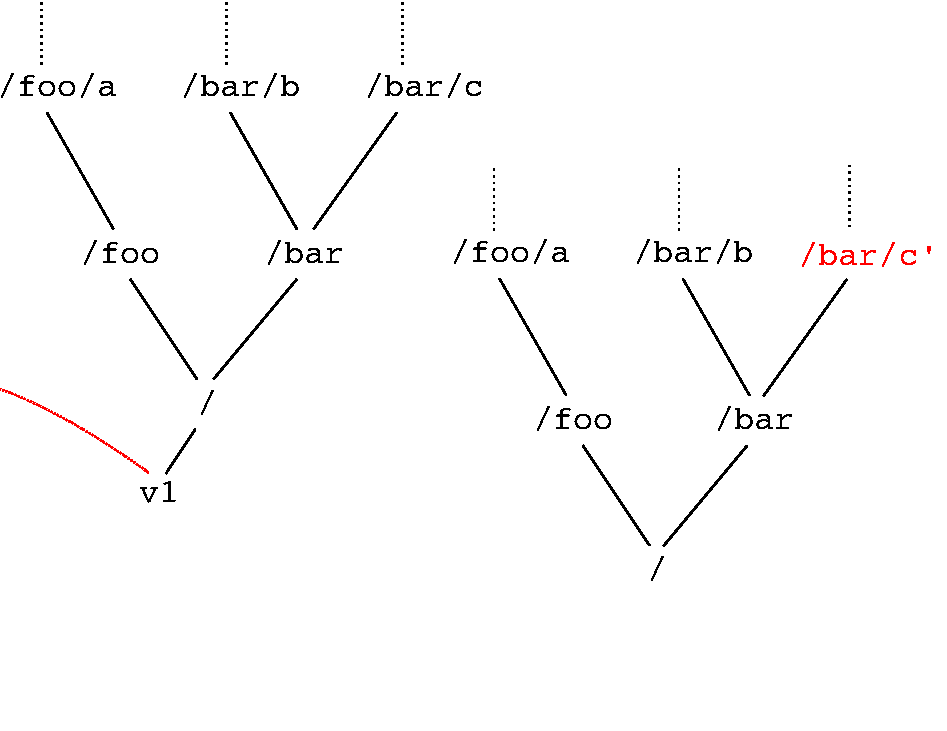
\includegraphics[width=0.85\textwidth]{images/git2.pdf}}%
      \only<+>{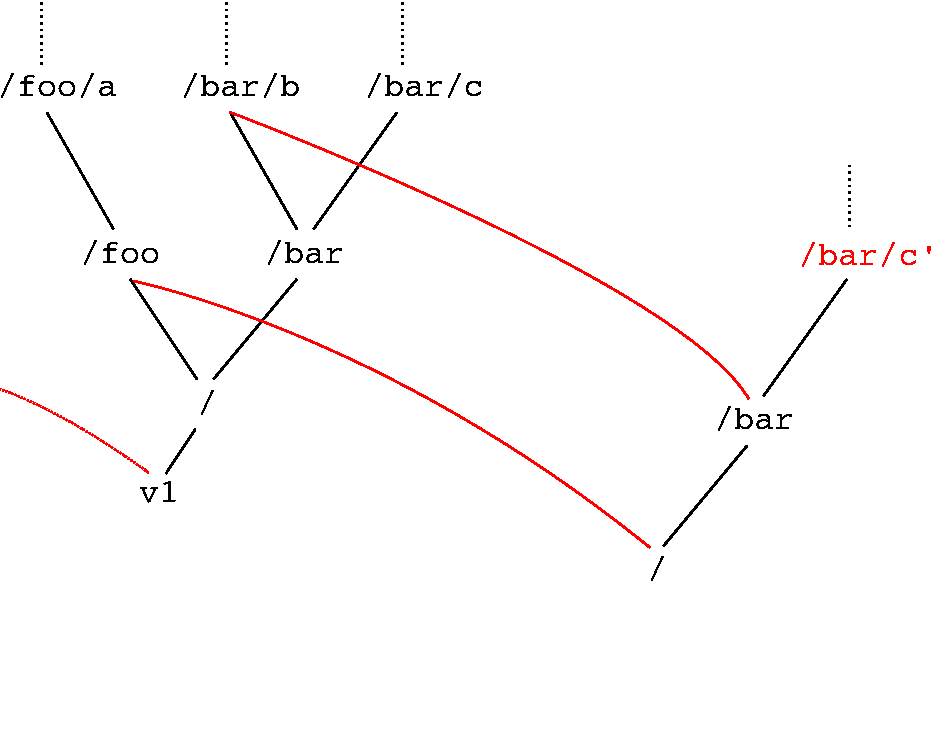
\includegraphics[width=0.85\textwidth]{images/git3.pdf}}%
      \only<+>{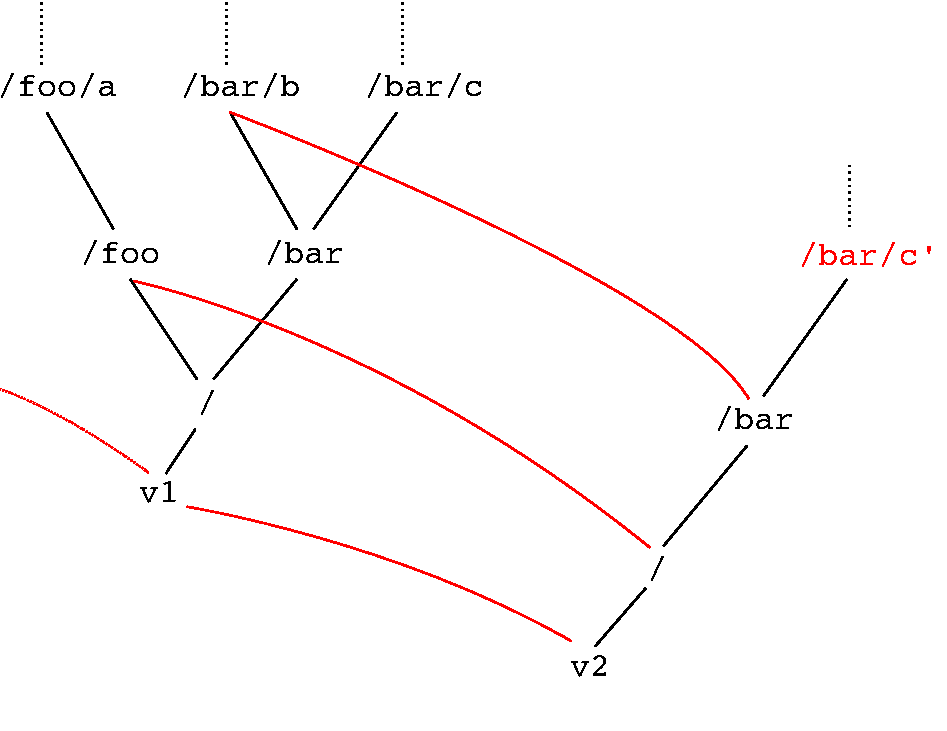
\includegraphics[width=0.85\textwidth]{images/git4.pdf}}%
      \only<+>{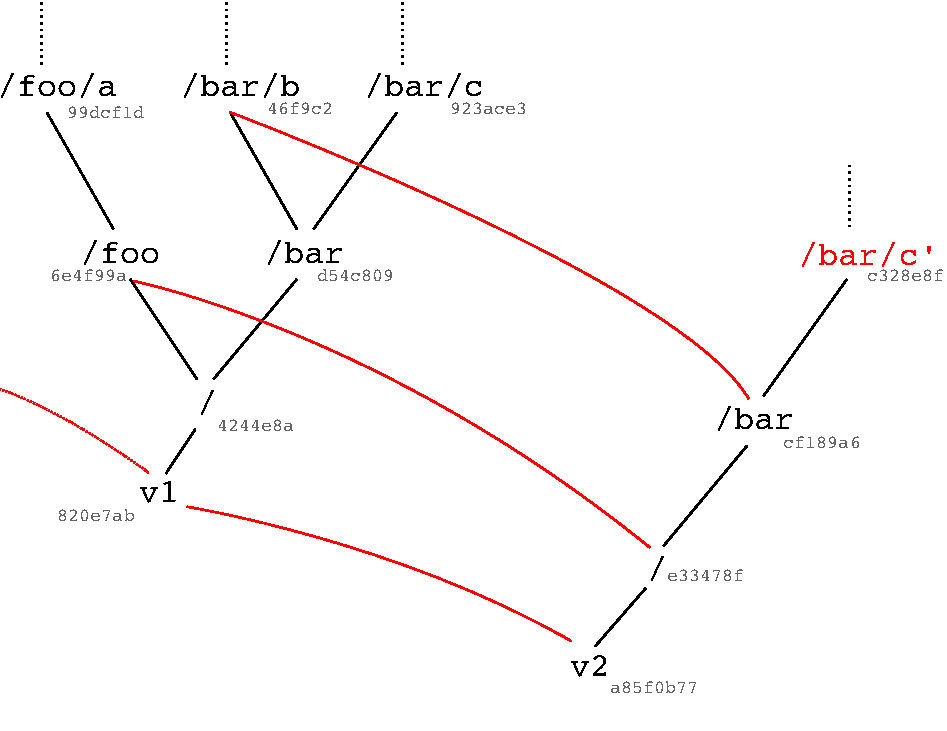
\includegraphics[width=0.85\textwidth]{images/git5.pdf}}%
      \only<+>{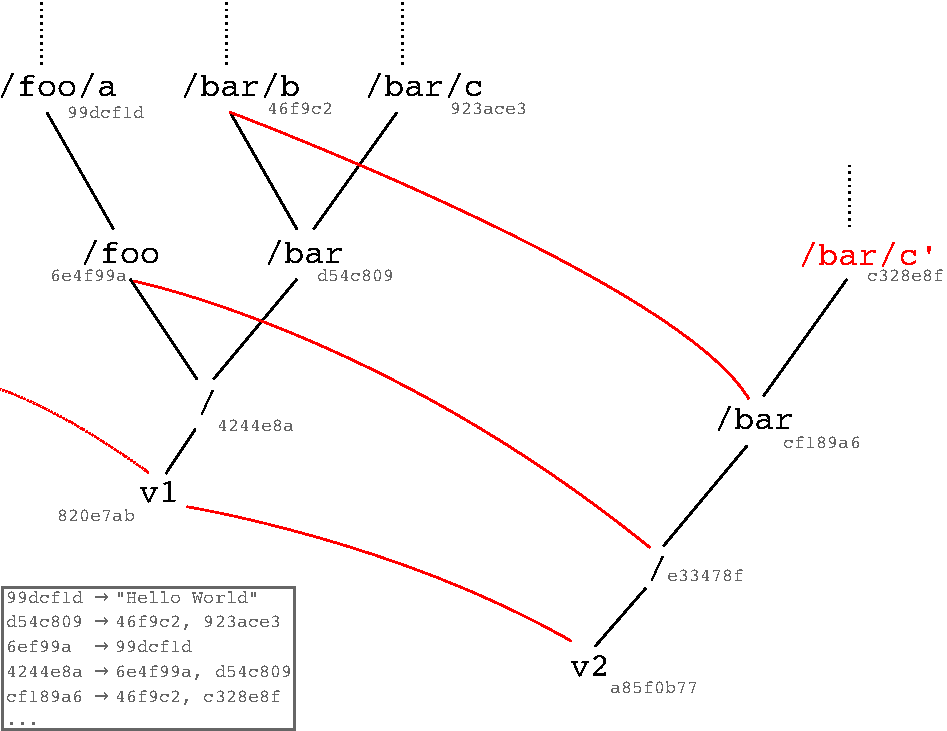
\includegraphics[width=0.85\textwidth]{images/git6.pdf}}%
      \only<+>{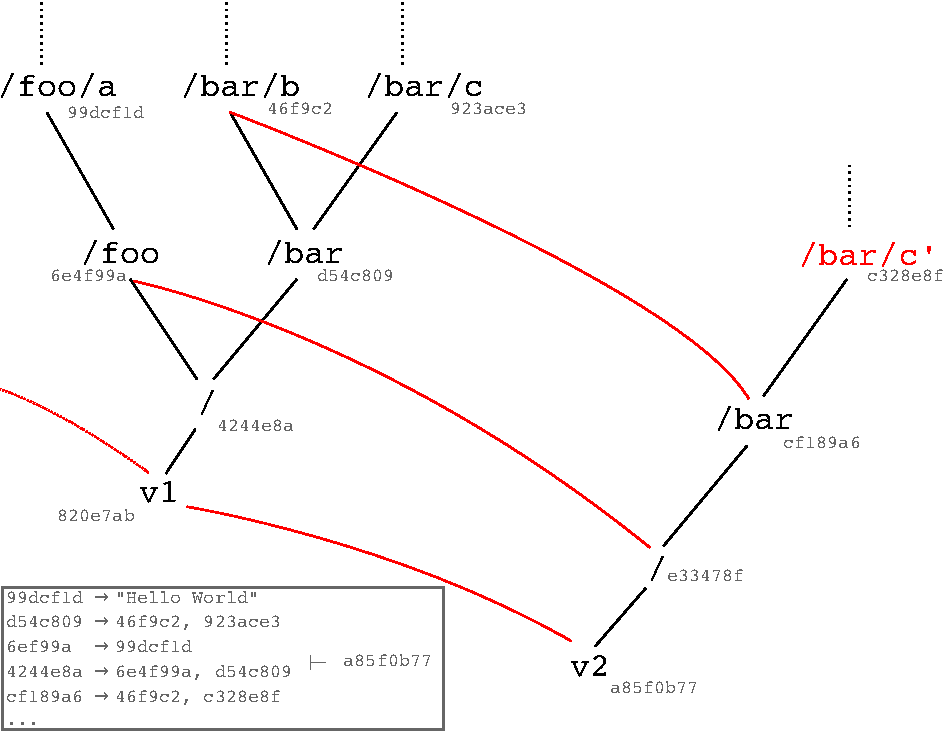
\includegraphics[width=0.85\textwidth]{images/git7.pdf}}%
    \end{center}
  \end{onlyenv}
  \begin{onlyenv}<8->
    The repository $R$ is a pair $(\Delta, x)$:
    \[ \Delta : x \mapsto (\mathsf{Commit}\ (x\times y) \gor \mathsf{Tree}\ \vec x
    \gor \mathsf{Blob}\ string)\]
    with the invariant:
    if $(x, \mathsf{Commit}\ (y,z)) \in\Delta$ then
    \begin{itemize}
    \item $(y, \mathsf{Tree}\ t)\in\Delta$
    \item $(z, \mathsf{Commit}\ (t,v))\in\Delta$
    \end{itemize}
    \pause
    \begin{center}
      \vspace{4em} {\Large Let's do the same with \emph{proofs}}
     \end{center}
  \end{onlyenv}
\end{frame}

\begin{frame}[fragile]{A \emph{typed} repository of proofs}
  \begin{onlyenv}<1-5>
    \begin{center}
      \only<+>{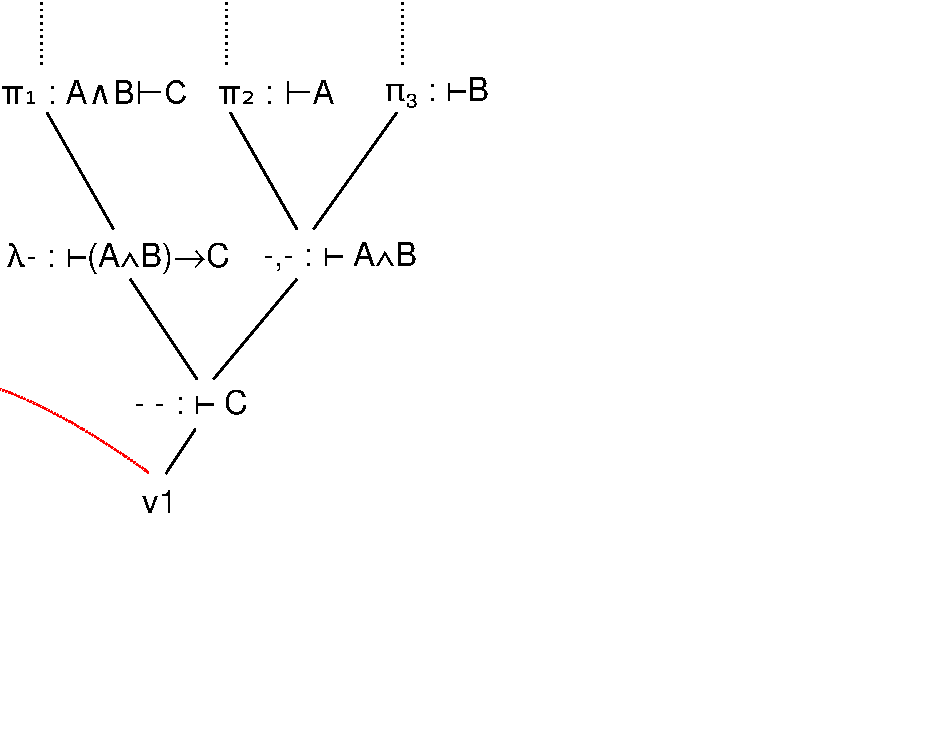
\includegraphics[width=0.85\textwidth]{images/gasp1.pdf}}%
      \only<+>{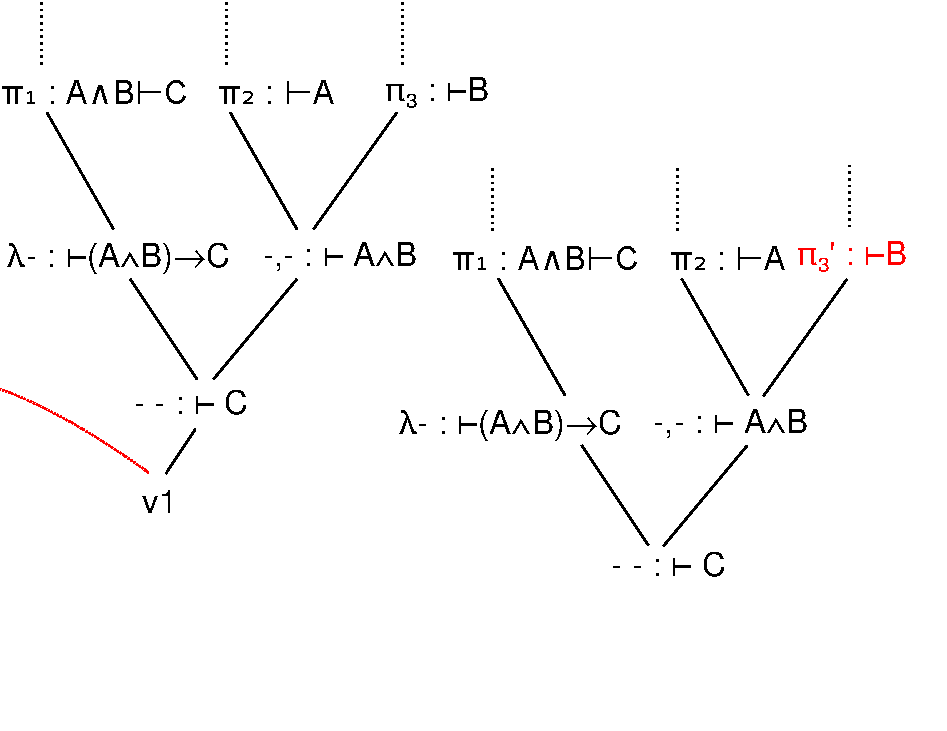
\includegraphics[width=0.85\textwidth]{images/gasp2.pdf}}%
      \only<+>{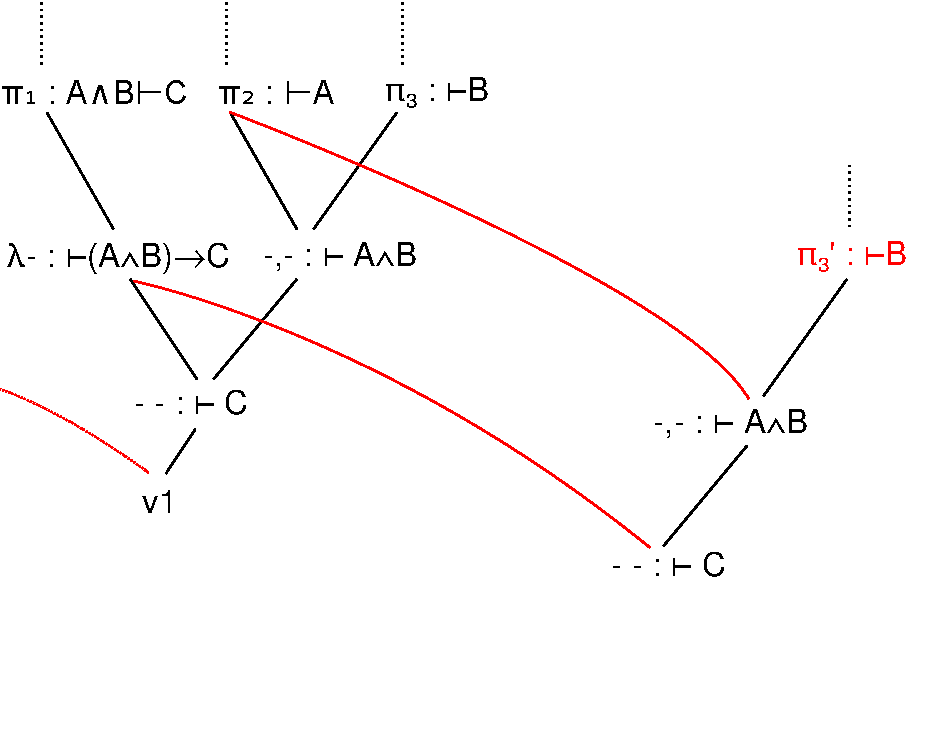
\includegraphics[width=0.85\textwidth]{images/gasp3.pdf}}%
      \only<+>{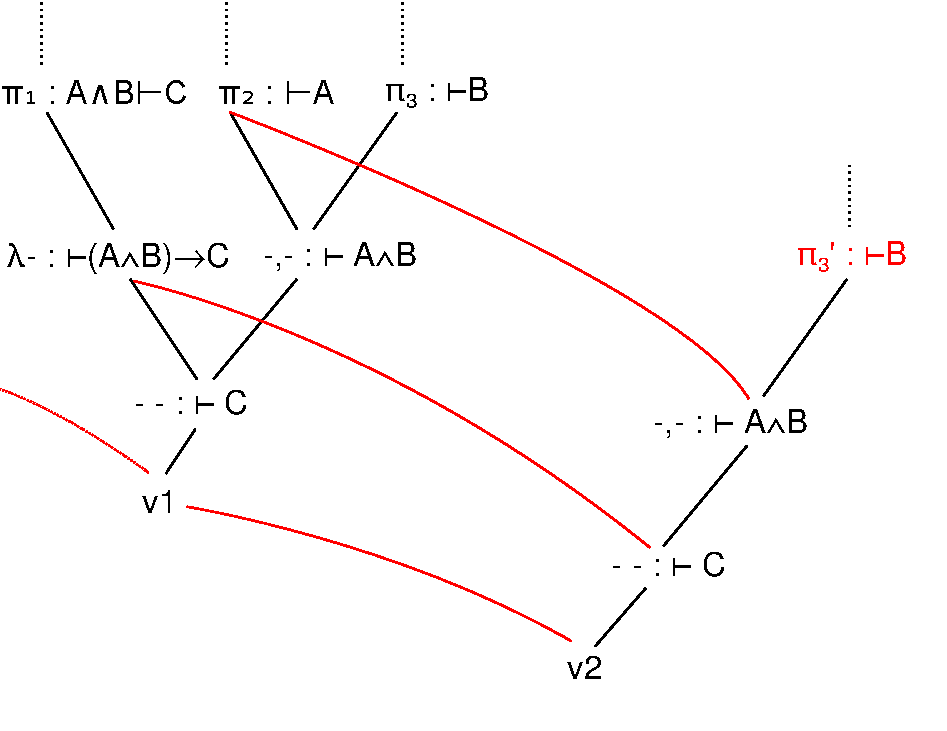
\includegraphics[width=0.85\textwidth]{images/gasp4.pdf}}%
      \only<+>{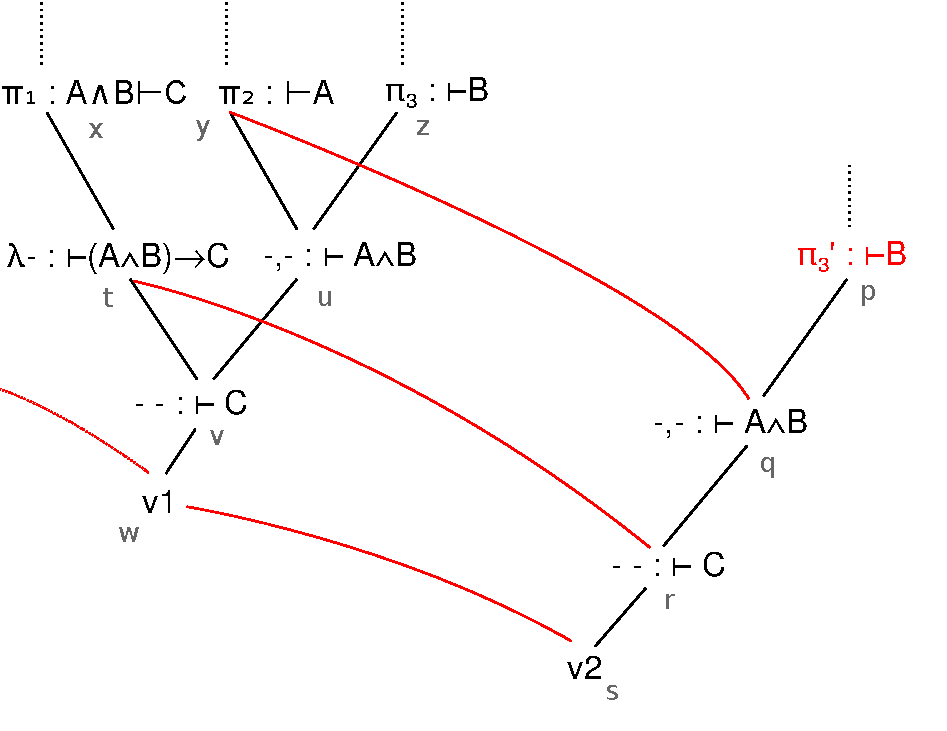
\includegraphics[width=0.85\textwidth]{images/gasp5.pdf}}%
    \end{center}
  \end{onlyenv}
  \begin{onlyenv}<6-9>
    \small
    \begin{overlayarea}{0pt}{\textheight}
      \begin{align*}
        x &= \ldots\ : A\wedge B\vdash C \\
        y &= \ldots\ :\ \vdash A \\
        z &= \ldots\ :\ \vdash B \\
        t &= \lam a {A\wedge B} x :\ \vdash A\wedge B\to C \\
        u &= (y, z) :\ \vdash A\wedge B \\
        v &= \app t u :\ \vdash C \\
        w &= \mathsf{Commit}(v,w1) : \mathsf{Version} \only<7>{
          \alert{\qquad,\quad w} }
        \only<8-9>{ \\
          p &=\ldots\ :\ \vdash B \\
          q &= (y, p) :\ \vdash A \wedge B \\
          r &= \app t q :\ \vdash C \\
          s &= \mathsf{Commit}(r,w) : \mathsf{Version} \only<9>{
            \alert{\qquad,\quad s} } }
      \end{align*}
    \end{overlayarea}
  \end{onlyenv}
  \begin{onlyenv}<10->
\footnotesize
\begin{uncoverenv}<12>
\begin{lstlisting}
...
val is : env -> prop -> type
val conj : prop -> prop -> prop
val pair : is 'a 'b -> is 'a 'c -> is 'a (conj 'b 'c)
val version : type
val commit : is nil C -> version -> version
...
\end{lstlisting}
\end{uncoverenv}
\begin{overlayarea}{\textwidth}{\textheight}
\begin{onlyenv}<10>
\begin{lstlisting}
let x = ... : is (cons (conj A B) nil) C in
  let y = ... : is nil A in
    let z = ... : is nil B in
      let t = lam (conj A B) x : is nil (arr (conj A B) C) in
        let u = pair y z : is nil (conj A B) in
          let v = app t u : is nil C in
            let w = commit v w1 : version in
              w
\end{lstlisting}
\end{onlyenv}
\begin{onlyenv}<11->
\begin{lstlisting}
let x = ... : is (cons (conj A B) nil) C in
  let y = ... : is nil A in
    let z = ... : is nil B in
      let t = lam (conj A B) x : is nil (arr (conj A B) C) in
        let u = pair y z : is nil (conj A B) in
          let v = app t u : is nil C in
            let w = commit v w1 : version in
              let p = ... : is nil B
                let q = pair y p : is nil (conj A B) in
                  let r = t q : is nil C
                    let s = commit r w : version in
                      s
\end{lstlisting}
\end{onlyenv}
\end{overlayarea}
  \end{onlyenv}
\end{frame}

\subsection{Logical framework}

\begin{frame}[fragile]{\gray{A} logical framework \gray{for incremental type-checking}}
  LF \cit{Harper et al. 1992} provides a way to represent and validate
  syntax, rules and proofs by means of a typed $\lambda$-calculus. But
  we need a little bit more: \\[1em]

  {\small\textsf{
      \noindent\ldots\\
      \alert<2>{\textbf{let}} \alert<5>u = \alert<4>{pair y z} : \alert<3>{is nil (conj A B)} \textbf{in}\\
      \hspace{2ex}\textbf{let} \alert<5>v = app t u : is nil C \textbf{in}\\
      \ldots
  }}
\pause
\begin{enumerate}[<+->]
\item definitions / explicit substitutions
\item type annotations on application spines
\item fully applied constants / $\eta$-long NF
\item Naming of all application spines / A-normal form\\
  {\footnotesize(= construction of syntax/proofs)}
\end{enumerate}

\end{frame}

\subsection{Positionality}

\begin{frame}[fragile]{Positionality}
$R =$ \scriptsize
\begin{lstlisting}
    let x = ... : is (cons (conj A B) nil) C in
      let y = ... : is nil A in
        let z = ... : is nil B in
          let t = lam (conj A B) x : is nil (arr (conj A B) C) in
            let u = pair y z : is nil (conj A B) in
              let v = app t u : is nil C in
                let w = commit v w1 : version in
                  w
\end{lstlisting}
\normalsize
\pause
\begin{itemize}
\item Expose the \emph{head} of the term
\pause {\Large \[(\lambda x y. T) U V\]}
\item \pause Abstract from the \emph{positions} of the binders \\
  {\footnotesize (from inside and from outside)}
\end{itemize}
\end{frame}

\section{The language}

\begin{frame}{Presentation}
  \begin{itemize}
  \item alternative syntax for LF
  \item a datastructure of LF derivations
  \item the repository storage model
  \end{itemize}
  \vspace{2em}
  \large
  \[
  \lambda_{\text{LF}}
  \quad\xrightarrow{\text{
      \begin{minipage}{20ex}
        \begin{center}
          LJ-style\\
          annotation
        \end{center}
      \end{minipage}
    }}\quad
  \text{XLF}
  \quad\xrightarrow{\text{
      \begin{minipage}{20ex}
        \begin{center}
          heads exposed\\
          forget positions
        \end{center}
      \end{minipage}
    }}\quad
  \text{NLF}
  \]
\end{frame}

\subsection{From LF to NLF}

\begin{frame}{From LF to XLF}
  \begin{overlayarea}{0em}{12em}
    \begin{align*}
      K &\gequal \prd x A K \gor \type \\
      A &\gequal \prd x A A \gor \alta{1}{2}{\app A t}
      {\alta{2}{3}{\lapp A l}{\laapp A l K}} \gor \alta{1}{2}{a}
      {\alta{2}{3}{\lapp a l}{\laapp a l K}} \\
      t &\gequal \lam x A t \gor \letb x t t \gor \alta{1}{2}{\app t
        t} {\alta{2}{3}{\lapp t l}{\laapp t l A}} \gor \alta{1}{2}{x}
      {\alta{2}{3}{\lapp x l}{\laapp x l A}} \gor \alta{1}{2}{c}
      {\alta{2}{3}{\lapp c l}{\laapp c l A}} \\
      \only<2->{\alert<2>l &\alert<2>{\gequal \lnil \gor
        \alta{5}{6}{\lcons t l}{\lncons x t l}}\\}
      \Gamma &\gequal \enil \gor \econs\Gamma{x:A} \gor \econs\Gamma{x=t} \\
      \Sigma &\gequal \enil \gor \econs\Sigma{c:A} \gor \econs\Sigma{a:K} \\
    \end{align*}
  \end{overlayarea}

  \begin{overlayarea}{\textwidth}{8em}
    \begin{itemize}[<+->]\small
    \item start from standard $\lambda_{LF}$ with definitions
    \item sequent calculus-like applications ($\bar\lambda$)
    \item type annotations on application spines
    \item<6-> named arguments
    \end{itemize}
    \small
    \only<4-6>{
        \begin{mathpar}
          \infer { \Gamma\vdash t : A \\ \alta{4}{5}{\Gamma,B\subst
              x t}{\econs\Gamma{x=t}, B}\vdash l : C} {\Gamma,\prd x A
            B \vdash \alta{5}{6}{\lcons t l}{\lncons x t l} : C}
        \end{mathpar}
      }
      \only<7->{
        \begin{align*}
          \FV{\laapp t l A} &= \FV{t} \cup \FV{l} \cup (\FV{A} - \FV{l}) \\
          \FV{\lncons x t l} &= \FV{t} \cup (\FV{l} - \{x\})
        \end{align*}
      }
  \end{overlayarea}
  \pause\pause
\end{frame}

\begin{frame}{XLF: Properties}
  \begin{itemize}
  \item LJ-style application
  \item type annotation on application spines
  \item named arguments (labels)
  \end{itemize}
  \begin{lemma}[Conservativity]
    \begin{itemize}
    \item $\jlfK \Gamma K \quad\text{iff}\quad \jxlfK {|\Gamma|} {|K|}$
    \item $\jlfA \Gamma A \quad\text{iff}\quad \jxlfA {|\Gamma|} {|A|}$
    \item $\jlft \Gamma t A \quad\text{iff}\quad \jxlft {|\Gamma|} {|t|} {|A|}$
    \end{itemize}
  \end{lemma}
\end{frame}

\begin{frame}{From XLF to NLF}
  \begin{overlayarea}{0em}{15.7em}
    \begin{align*}
      K &\gequal \alta{9}{10}{\prd x A K \gor \alta{1}{2}{\type}{h_K}}{\Gamma\vdash h_k} \\
      \only<2->{\alert<2>{h_K}}\only<2->{&\alert<2>{\gequal \type} \\}
      A &\gequal \alta{8}{9}{ \prd x A A \gor \alta{2}{3}{\laapp A l K
          \gor \laapp a l K}{h_A}}
      {\Gamma\vdash h_A}\\
      \only<3->{\alert<3>{h_A} &\alert<3>{\gequal\laapp A l {\alta{4}{5} K
          {h_K}} \gor
        \laapp a l {\alta{4}{5} K {h_K}}} \\}
      t &\gequal \alta{7}{8}{\lam x A t \gor \letb x t t \gor
        \alta{3}{4}{\laapp t l A \gor \laapp x l A \gor
          \laapp c l A}{h_t}}{\Gamma\vdash h_t} \\
      \only<4->{\alert<4>{h_t}&\alert<4>{\gequal \laapp t l
        {\alta{5}{6}{A}{h_A}} \gor \laapp x l {\alta{5}{6}{A}{h_A}}
        \gor
        \laapp c l {\alta{5}{6}{A}{h_A}}}\\}
      l &\gequal \alta{10}{11}{\lnil \gor
        \lncons x t l}{\Gamma} \\
      \alta{11}{12}\Gamma\Gamma &\alta{11}{12} {\gequal \enil \gor
        \econs\Gamma{x:A} \gor \econs\Gamma{x=t}}
      {\ :\ x \mapsto (\eent{x:A} \gor \eent{x=t})} \\
      \Sigma &\gequal \enil \gor \econs\Sigma{c:A} \gor \econs\Sigma{a:K} \\
    \end{align*}
  \end{overlayarea}
  \begin{itemize}[<+->] \small
  \item start from XLF
  \item isolate heads (non-binders) \pause\pause
  \item enforce $\eta$-long forms by annotating with heads \pause
    \only<+>{\[
    \laapp t l {\prd x A B}\quad\too_\eta\quad \lam x A ({\laapp t
      {x=x;l} B}) \qquad \notinfv{x}{t}
    \]}
  \item factorize binders and environments \pause\pause\pause
  \item abstract over environment datastructure (maps)
  \end{itemize}
\end{frame}

\subsection{NLF: Syntax, typing, reduction}

\begin{frame}{NLF}
  \begin{block}{Syntax}
    \begin{align*}
      \\[-3em]
      K &\gequal \jnlfK\Gamma \\
      A &\gequal \jnlfA\Gamma{h_A} \\
      h_A &\gequal \app a \Gamma \\
      t &\gequal \jnlft\Gamma{h_t}{h_A} \\
      h_t &\gequal \app t\Gamma \gor
      \app x\Gamma \gor \app c\Gamma \\
      \Gamma &\quad :\quad x \mapsto (\eent{x:a} \gor \eent{x=t})
    \end{align*}
  \end{block}
  \begin{overlayarea}{\textwidth}{\textwidth}
    \begin{block}{Judgements}
      \begin{itemize}
      \item $\alt<-1>{\jnlfK\Gamma}{\alt<-2> K {\jwf K}}$
      \item $\alt<-1>{\jnlfA\Gamma{h_A}}{\alt<-2> A {\jwf A}}$
      \item $\alt<-1>{\jnlft\Gamma{h_t}{h_A}}{\alt<-2> t {\jwf t}}$
      \end{itemize}
    \end{block}
  \end{overlayarea}
  \pause\pause
\end{frame}

\begin{frame}{NLF}
  \begin{block}{Notations}
    \begin{itemize}
    \item ``$h_A$'' for ``$\empty\vdash h_A$''
    \item ``$h_A$'' for ``$\jnlfA{\emptyset}{h_A}$''
    \item ``$a$'' for ``$\app a \emptyset$''
    \end{itemize}
  \end{block}
  \begin{example}
    $\lam f {A\to B} \lam x A \app f x : (A\to B)\to A\to B\qquad\equiv$\\[0.5em]
    $\jnlft
    {\econs
      {\eent{f:\jnlfA{\eent{a:A}}{B}}}
      {x:A}}
    {\app f {\esing{a=x}}}
    {B}$
  \end{example}
\end{frame}

\begin{frame}{Some more examples}
  \begin{enumerate}
  \item[$A:$] $\jnlfK\emptyset$
    \begin{smallright}
      $\equiv \type$
    \end{smallright}
  \item[$vec:$]
    $\jnlfK{\esing{len:\nat}}$
    \begin{smallright}
      $\equiv \nat\to\type$
    \end{smallright}
  \item[$nil:$]
    $\jnlfA{}{\app{vec}\esing{len=\jnlft{}{0}{\nat}}}$
    \begin{smallright}
      \footnotesize $\equiv \app{vec} 0 : \type$
    \end{smallright}
  \item[$cons:$]
    $\jnlfA { \econs{ \econs{ \esing{l:\nat}} {hd:A}}
      {tl:\jnlfA{}{ \app {vec} {\esing{len=\jnlft{}{l}{\nat}}}}}}
    {\app{vec} {\esing{len =\jnlft{}{\app s {\esing{n =
                \jnlft{}{l}{\nat}}}}{\nat}}}}$
    \begin{smallright}
      $\equiv \prd l \nat A\to \prd {tl} {\app {vec} l}
      \app {vec} (\app s l : \nat) : \type$
    \end{smallright}
  \item[$fill:$]
    $\jnlfA{\esing{n:\nat}}{\app{vec}{\esing{len=\jnlft{}{n}{\nat}}}}$
    \begin{smallright}
      $\equiv \prd n \nat (\app{vec} n : \type)$
    \end{smallright}
  \item[$empty:$]
    $\jnlfK{\esing{e:\app{vec}\esing{len=0}}}$
    \begin{smallright}
      $\equiv \app{vec} 0\to \type$
    \end{smallright}
  \item[$-:$]
    $\jnlfA{}{\app{empty}\esing{e=\jnlft{}{\app{fill}\esing{n=0}}{\app{vec}\esing{len=n}}}}$
    \begin{smallright}
      $\equiv \app{empty}(\app{fill} 0 : \app{vec} 0)$
    \end{smallright}
  \end{enumerate}
\end{frame}

\begin{frame}{Environments}
  \ldots\ double as labeled \emph{directed acyclic graphs} of
  dependencies:
  \begin{overlayarea}{\textwidth}{\textheight}
    \only<1>{
      \begin{definition}[environment]
        $\Gamma = (V,E)$ directed acyclic where:
        \begin{itemize}
        \item $V \subseteq \mathcal X \times (t \uplus A)$ and
        \item $(x,y)\in E$ ($x$ depends on $y$) if
          $y\in\FV{\elookup\Gamma x}$
        \end{itemize}
      \end{definition}
      \begin{definition}[lookup]
        $\elookupdecl\Gamma x A \quad\text{if}\quad (x,A)\in E$ \\
        $\elookupdef\Gamma x t \quad\text{if}\quad (x,t)\in E$
      \end{definition}
      \begin{definition}[bind]
        $\ebinddecl\Gamma x A = ( V\cup (x,A), E\cup\{(x,y)\ |\
        y\in\FV{A}\} )$ $\ebinddef\Gamma x t = ( V\cup (x,A),
        E\cup\{(x,y)\ |\ y\in\FV{t}\} )$
      \end{definition}
    } \only<2->{
      \begin{definition}[decls, defs]
        $\edecls\Gamma = [x_1,\ldots, x_n]$
        s.t. $\elookupdecl\Gamma{x_i}{A_i}$ topologically sorted
        \emph{wrt.} $\Gamma$\\
        $\edefs\Gamma = [x_1,\ldots, x_n]$
        s.t. $\elookupdef\Gamma{x_i}{t_i}$ topologically sorted
        \emph{wrt.} $\Gamma$
      \end{definition}
      \begin{definition}[merge]
        $\emerge\Gamma\Delta = \Gamma\cup\Delta$ s.t.
        \begin{itemize}
        % \item if $\elookupdecl\Gamma x A$ and $\elookupdecl\Gamma x B$
        %   then $\elookupdecl{\emerge\Gamma\Delta} x B$
        \item if $\elookupdecl\Gamma x A$ and $\elookupdef\Gamma x t$
          then $\elookupdef{\emerge\Gamma\Delta} x t$
        \item undefined otherwise
        \end{itemize}
      \end{definition}
    }
  \end{overlayarea}
\end{frame}

\begin{frame}{Reduction}
  
\end{frame}

\begin{frame}{Typing}
  \small
  \begin{mathpar}
    \infer[Fam]
    {\elookupdecl\Sigma a {(\jnlfK{\Xi})} \\
      \jnlfargs\Gamma\Delta\Xi
    }
    {\jnlfA\Gamma{\app a \Delta}}
    \and
    \infer[Objc]
    {\elookupdecl\Sigma c {(\jnlfA\Xi{h_A})} \\
      \jnlfargs\Gamma\Delta\Xi \\
      \jnlfconvA{\emerge{\emerge\Gamma\Xi}\Delta}{h_A'}{h_A}
    }
    {\jnlft\Gamma{\app c \Delta}{h_A'}}
    \and
    % \infer[Objx$_1$]
    % {\elookupdecl\Gamma x {(\jnlfA\Xi{h_A})} \\
    %   \jnlfargs\Gamma\Delta\Xi \\
    %   \jnlfconvA{\emerge{\emerge\Gamma\Xi}\Delta}{h_A'}{h_A}
    % }
    % {\jnlft\Gamma{\app x \Delta}{h_A'}}
    % \and\pause
    \infer[Objx]
    {\elookupdef\Gamma x {(\jnlft\Xi{h_t}{h_A})} \\
      \jnlfargs\Gamma\Delta\Xi \\
      \jnlfconvA{\emerge{\emerge\Gamma\Xi}\Delta}{h_A'}{h_A} \\\\
      \jnlft{\emerge{\emerge\Gamma\Xi}\Delta}{h_t}{h_A}
    }
    {\jnlft\Gamma{\app x\Delta}{h_A'}}
    \and
    \infer[Args ${\small\ {\forall x\in \edecls\Xi}}$]
    {
      \elookupdef\Delta x {(\jnlft{\Delta'}{h_t}{h_A})}\\
      \elookupdecl\Xi x {(\jnlfA{\Xi'}{h_A'})} \\
      \jnlft{\emerge{\emerge\Gamma\Delta}\Delta'}{h_t}{h_A} \\
      \jnlfconvA{\emerge{\emerge{\emerge{\emerge\Gamma\Xi}\Delta}\Xi'}\Delta'}{h_A'}{h_A}
    }
    {\jnlfargs\Gamma\Delta\Xi}
  \end{mathpar}
\end{frame}

% \begin{frame}{Conversion}
%   \begin{mathpar}
%     \infer[ConvFam]
%     {\jnlfconve\Gamma\Delta\Xi}
%     {\jnlfconvA\Gamma{\app a \Delta}{\app a \Xi}}
%     \and\pause
%     \infer[ConvObjc]
%     {\jnlfconve\Gamma\Delta\Xi}
%     {\jnlfconvt\Gamma{\app c\Delta}{\app c\Xi}{h_A}}
%     \and\pause
%     \infer[ConvArgs ${\small\ \forall x\in \edefs\Xi\cap\edefs\Delta}$]
%     {
%       \elookupdef\Delta x {\jnlft{\Delta'}{h_t}{h_A}}\\
%       \elookupdef\Xi x {\jnlft{\Xi'}{h_t'}{h_A'}} \\
%       \jnlfconvA{\emerge{\emerge{\emerge{\Gamma\Delta}\Xi}\Delta'}\Xi'}{h_A}{h_A'}
%       \\
%       \jnlfconvt{\emerge{\emerge{\emerge{\Gamma\Delta}\Xi}\Delta'}\Xi'}{h_t}{h_t'}{h_A}
%     }
%     {\jnlfconve\Gamma\Delta\Xi}
%     \\\pause
%     \ldots
%   \end{mathpar}
% \end{frame}


\begin{frame}{Properties}
  \begin{block}{Translation functions}
    \begin{itemize}
    \item $|\cdot|_\Gamma\ :\ K_{\mathrm{LF}} \to
      \Gamma_{\mathrm{NLF}} \to K_{\mathrm{NLF}}\ \mathsf{option}$
    \item $|\cdot|_\Gamma\ :\ A_{\mathrm{LF}} \to
      \Gamma_{\mathrm{NLF}} \to A_{\mathrm{NLF}}\ \mathsf{option}$
    \item $|\cdot|_\Gamma\ :\ t_{\mathrm{LF}} \to
      \Gamma_{\mathrm{NLF}} \to t_{\mathrm{NLF}}\ \mathsf{option}$
    \item \ldots\ and their inverses $|\cdot|^{-1}$
    \end{itemize}
  \end{block}
  \begin{block}{Conjecture (Conservativity)}
    \begin{itemize}
    \item $\jlfK {} K \quad\text{iff}\quad \jwf{(|K|_\emptyset)}$
    \item $\jlfA {} A \quad\text{iff}\quad \jwf{(|A|_\emptyset)}$
    \item $\jlft {} t A \quad\text{iff}\quad \jwf{(|t|_\emptyset)} $
    \end{itemize}    
  \end{block}
\end{frame}

\section{Architecture}

\begin{frame}[fragile]{Status}
\small
\begin{verbatim}
$ ./gasp init hol.elf
\end{verbatim}
\pause
\begin{verbatim}
[holtype : kind]
[i : holtype]
[o : holtype]
[arr : [x2 : holtype][x1 : holtype] ⊢ holtype type]

Fatal error: exception Assert_failure("src/NLF.ml", 61, 13)
\end{verbatim}
\end{frame}

\begin{frame}[fragile]{Checkout}
\small
\begin{verbatim}
$ ./gasp checkout v42
\end{verbatim}
\normalsize
if
\[t = \Gamma\vdash v_{52} : \mathsf{Version} \quad\text{and}\quad
\Gamma(v_{42}) = \mathsf{Commit}(v_{41},h) \]
then 
\[ |\Gamma(h)|^{-1} \]
is the LF term representing \texttt{v42}
\end{frame}

\begin{frame}[fragile]{Commit}
  \small
\begin{verbatim}
$ ./gasp commit term.elf
\end{verbatim}
\normalsize
if
\[ t = \Gamma\vdash v_{52} : \mathsf{Version} \quad\text{and}\quad
|\mathtt{term.elf}|_\Gamma = \Delta\vdash h_t:h_A \]
then 
\[ \econs\Delta{v_{53} = \app{\mathsf{Commit}} \econs{\esing{prev =
      v_{52}}}{this = h_t}}\vdash v_{53} : \mathsf{Version}\] is the
new repository
\end{frame}

\begin{frame}{Further work}
  \begin{itemize}
  \item still some technical \& metatheoretical unknowns
  \item from derivations to terms (proof search? views?)
  \item \textsf{diff} on terms or derivations
  \item type errors handling and recovery
  \item mimick other operations from VCS (\textsf{Merge})
  \end{itemize}
\end{frame}

\end{document}
